\documentclass{beamer}


\usepackage{amsmath}
\usepackage[style=alphabetic,url=true]{biblatex}
\usepackage{environ}
\usepackage{geometry}
\usepackage{graphicx}
\usepackage{tikz}
\usepackage[T2A]{fontenc}
\usepackage[utf8]{inputenc}
\usepackage[cache=false]{minted}
\usepackage{amsmath}
\usepackage{amsfonts}
\usepackage{amssymb}
\usepackage{calrsfs}


% \usetheme{Bergen}

\usecolortheme{beaver}

\setbeamertemplate{itemize item}[circle]
\setbeamertemplate{itemize subitem}{--}
\addtobeamertemplate{navigation symbols}{}{
  \usebeamerfont{footline}%
  \usebeamercolor[fg]{footline}%
  \hspace{1em}%
  \insertframenumber/\inserttotalframenumber
}
\graphicspath{ {./graphics/} }
\setminted[Python]{
  fontsize=\tiny
}
\BeforeBeginEnvironment{minted}{\medskip}
\AfterEndEnvironment{minted}{\medskip}



\title{
  Bitcoin and Cryptocurrency Technologies \\
  Lecture 2: Cryptography Basics 1/2
}

\author{Yuri Zhykin}
\date{Feb 15, 2022}

\begin{document}

\frame{\titlepage}

\begin{frame}
  \frametitle{Introduction to Cryptography}
  \begin{itemize}
  \item \textbf{Cryptography} (Ancient Greek, ``hidden, secret'' and ``to
    write''), is the practice and study of techniques for \textit{secure
      communication} in the \textit{presence of \textbf{third parties} called
      adversaries}.
  \item \textbf{Modern cryptography} is heavily based on \textit{mathematical
      theory and computer science practice}.
  \item \textbf{Modern cryptographic algorithms} are designed around
    computational hardness assumptions.
  \end{itemize}
\end{frame}

\begin{frame}
  \frametitle{Introduction to Cryptography 2/2}
  \begin{itemize}
  \item Modern cryptography is divided into two categories:
    \begin{itemize}
    \item \textbf{symmetric cryptography} - both parties share the same secret
      key, used for both encryption and decryption,
    \item \textbf{asymmetric (public-key) cryptography} - key consists of public
      and private components; public key is used for encryption, private key -
      for decryption.
    \end{itemize}
  \item Cryptography protocols serve two main purposes:
    \begin{itemize}
    \item \textbf{concealing communication} (encryption/decryption),
    \item \textbf{ensuring integrity of communication} (signing/signature
      verification)
    \end{itemize}
  \end{itemize}
\end{frame}

\begin{frame}
  \frametitle{Symmetric Cryptography}
  \begin{itemize}
  \item The only type of cryptography until 1976.
  \item Both parties have a shared secret key that is used for both encryption
    and decryption.
  \item Symmetric encryption alrgorithms are very fast (e.g. \textit{AES},
    \textit{Salsa20}, \textit{ChaCha}).
  \item Most popular symmetric encryption algorithms are implemented in hardware
    (e.g. \textit{AES} and AES-NI instruction set for x86 CPUs).
  \item Perfect encryption scheme:
    \begin{align*}
      &E = M \oplus K, \\
      &D = E \oplus K, \\
      &|M| == |K|
    \end{align*}
  \end{itemize}
\end{frame}

\begin{frame}
  \frametitle{Symmetic Cryptography Problems}
  \begin{itemize}
  \item Secret key must be shared beforehand over a secure communication channel
    - ``chicken-and-egg'' problem.
  \item Symmetry of failure - if any of the parties leaks the key, both parties
    are compromised.    
  \item If multiple parties share the same key, the symmetry of failure affects
    all parties.  
  \item If each party keeps a different key for each other party (ideally), key
    storage is yet another problem.
  \end{itemize}
\end{frame}

\begin{frame}
  \frametitle{Public-key Cryptography}
  \begin{itemize}
  \item Groundbreaking discovery by \textbf{Whitfield Diffie} and \textbf{Martin
      Hellman} in 1976.
  \item Messages are encrypted with public key, but can only be decrypted with
    the private key.
  \item Each party is responsible only for its own private key - public key can
    be derived from it, if lost, and can be exchanged over insecure
    communication channels
  \end{itemize}
\end{frame}

\begin{frame}[fragile]
  \frametitle{Probability, Randomness and Large Numbers 1/3}
  \begin{itemize}
  \item In most modern cryptographic systems, the security of the keys is based
    on probability of guessing very large numbers.
  \item In order to make this as hard as possible, the numbers must be truly
    random, i.e. the probability of each bit in the number to be either 1 or 0
    must be 0.5.
  \item Probability of guessing a truly random number $N$ is exactly $1/N$.
  \item The estimated number of atoms in the Universe is
    $10^{78} \simeq 2^{259}$, so guessing a 256-bit key is almost equivalent to
    guessing a particular atom in the Universe.
  \end{itemize}
\end{frame}

\begin{frame}[fragile]
  \frametitle{Probability, Randomness and Large Numbers 2/3}
  \begin{itemize}
  \item At the same time, large numbers used as keys can be compactly
    represented with hexadecimal (base-16) or base-64 encodings:
\begin{minted}{Python}
import secrets
import base64
bits = secrets.randbits(256)
# 46518555179467323509970270980993648640987722172281263586388328188640792550961
bits_binary = '{0:b}'.format(bits)
# 110011011011000100100011011010111101101011111110101000111100101000001000100101\
# 111100110101001111110101111100100111000101110101011100011001010111001011000001\
# 111010110101010000010001000001111110111110011000000110011100100111111010110100\
# 100100001111000110001
bits_hex = hex(bits)
# 0x66d891b5ed7f51e5044be6a7ebe4e2eae32b960f5aa0883f7cc0ce4fd6921e31
bits_base64 = base64.b64encode(bits.to_bytes(32, 'little'))
# MR6S1k/OwHw/iKBaD5Yr4+ri5Oun5ksE5VF/7bWR2GY=
\end{minted}
  \end{itemize}
\end{frame}

\begin{frame}[fragile]
  \frametitle{Probability, Randomness and Large Numbers 3/3}
  \begin{itemize}
  \item Computers are deterministic, so generating truly random numbers is hard.
  \item In most cases, the most secure way to get a random number on Unix
    systems is to read from \mintinline{Bash}{/dev/random} or
    \mintinline{Bash}{/dev/urandom} devices.
  \item Special hardware exists for generating truly random numbers based on
    environment entropy; they should be preferred if possible.
  \end{itemize}
\end{frame}

\begin{frame}
  \frametitle{Hash Functions}
  \begin{itemize}
  \item \textbf{Hash function} is a function that maps data of arbitrary size to
    fixed-size values.
  \item Hash functions are used for storage adressing (hash tables),
    probabilistic filtering (bloom filters), etc.
    \begin{center}
      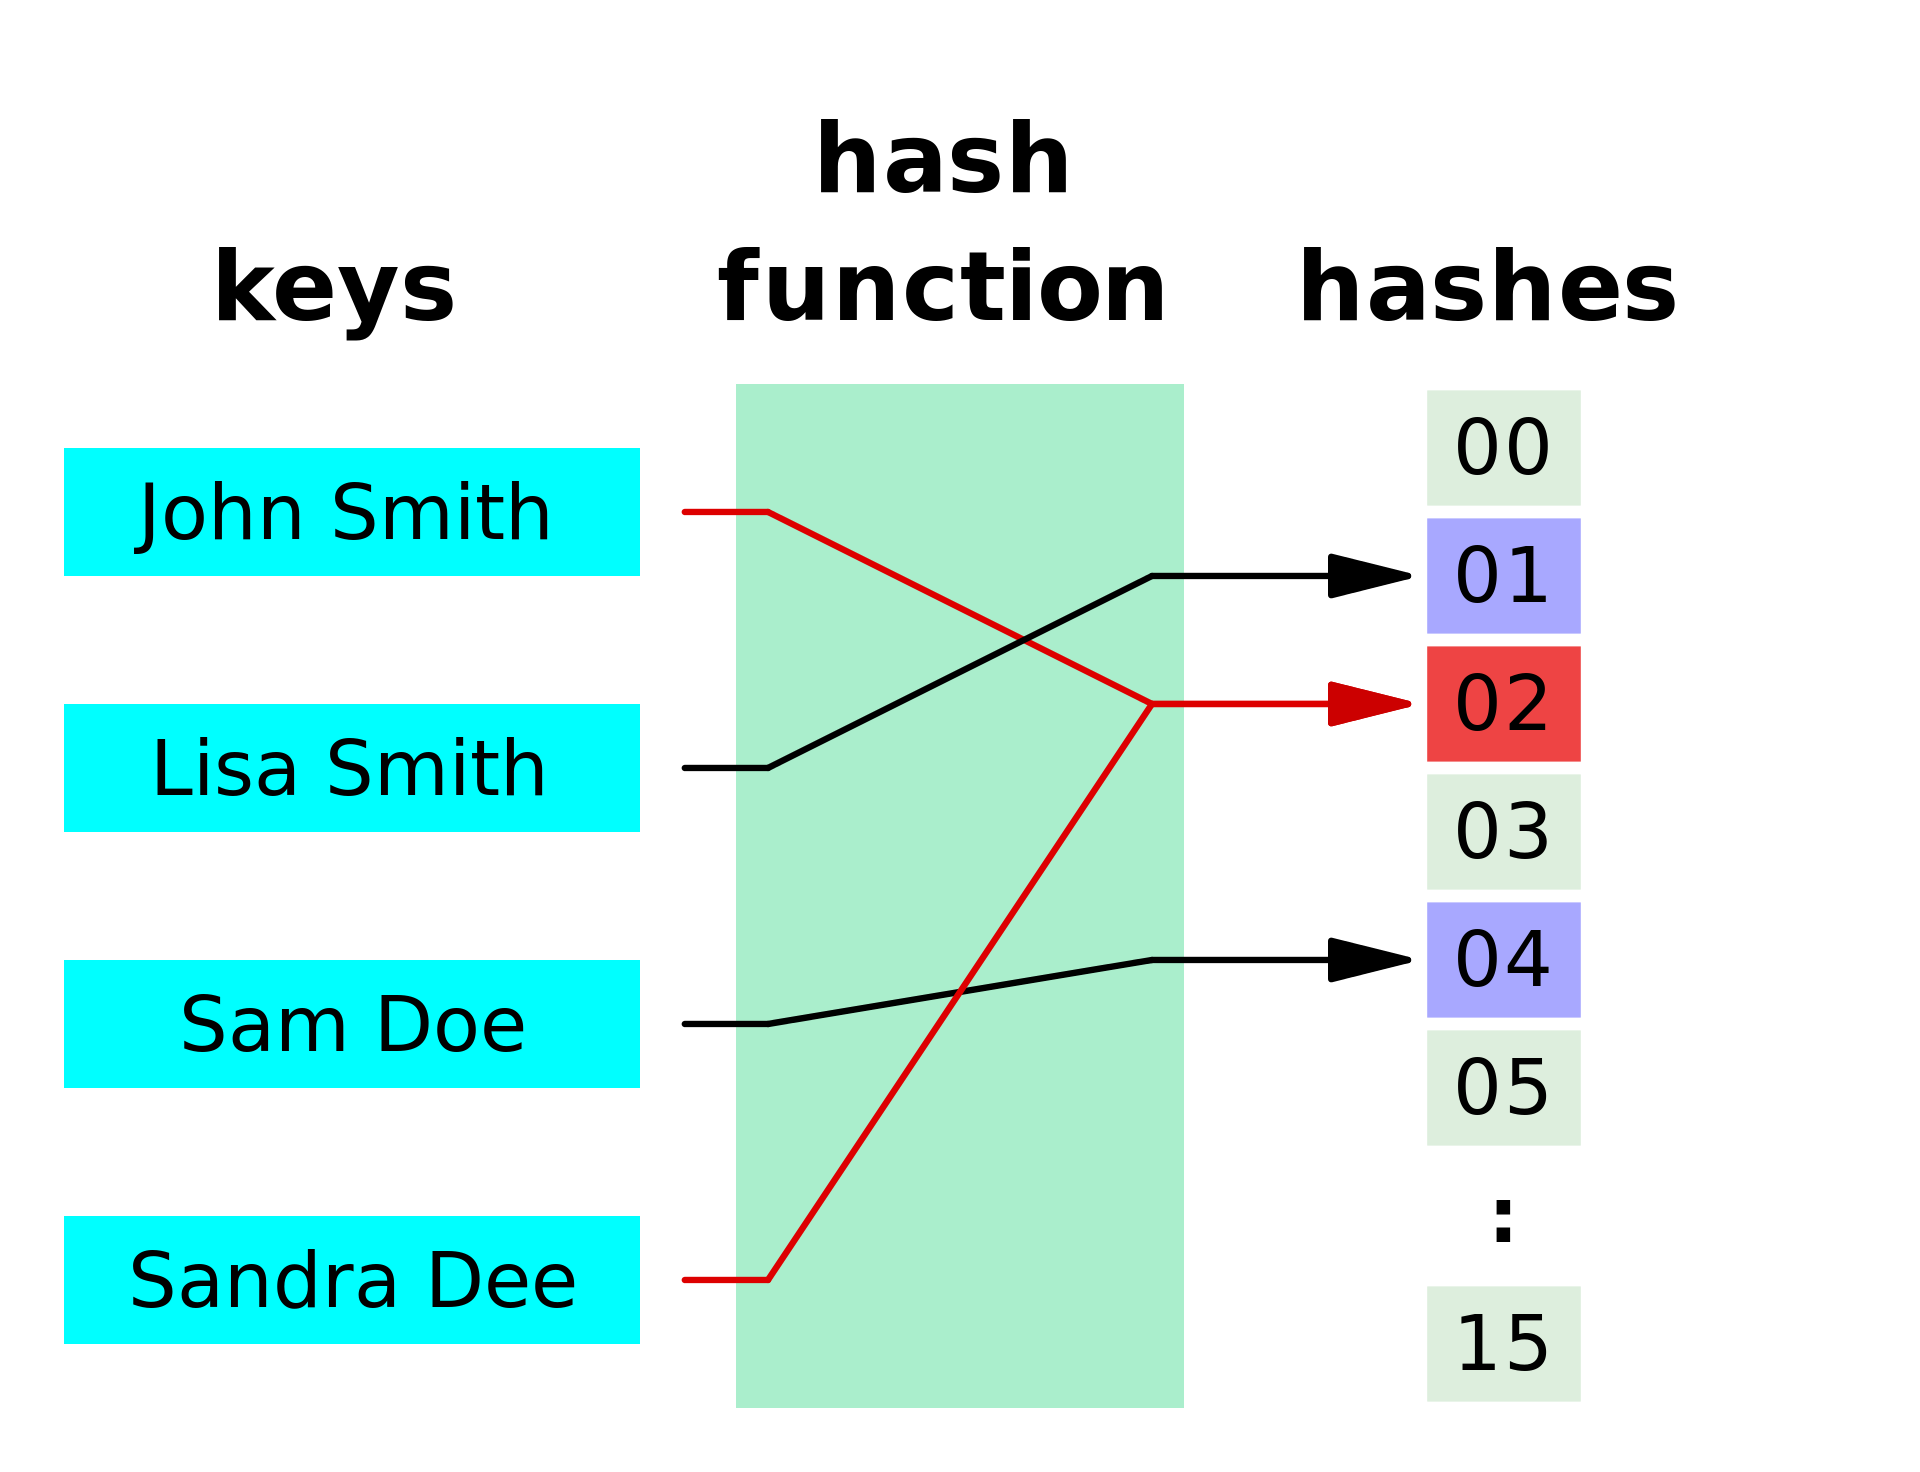
\includegraphics[width=0.6\textwidth,]{hash_function}
    \end{center}
  \end{itemize}
\end{frame}

\begin{frame}
  \frametitle{Cryptographic Hash Functions}
  \begin{itemize}    
  \item \textbf{Cryptographic hash function} is a \textit{hash function} that
    maps data to bit arrays of fixed size and is a \textbf{one-way function},
    that is, a function that is practically infeasible to invert:
    \begin{align*}
      h = H(m)&\text{ - efficient,}\\
      m = H^{-1}(h)&\text{ - \textbf{very} inefficient}
    \end{align*}
  \item The \textbf{most efficient} way to find a message $m$ that produces a
    given hash $h$ is a \textbf{brute-force search} - generate random messages
    $m_i$ and check if $H(m_i) = h$.
  \item Basic tool of modern cryptography.
  \end{itemize}
\end{frame}

\begin{frame}
  \frametitle{Properties of Cryptographic Hash Functions}
  \begin{itemize}
  \item Main properties of \textbf{good} cryptographic hash functions:
    \begin{itemize}
    \item \textbf{determinism} - same input always produces same output,
    \item \textbf{efficiency} - hash of a given message can be computed quickly,
    \item \textbf{diffusion, ``avalanche effect''} - a single-bit change in $m$
      causes change of every bit in $h$ with probability 0.5,
    \item \textbf{pre-image resistance} - given hash $h$, it should be hard to
      find any message $m$ such that $h = H(m)$,
    \item \textbf{second pre-image resistance} - given input $m_1$, it should be
      hard to find any $m_2$ such that $H(m_1) = H(m_2)$,
    \item \textbf{collision resistance} - it should be hard to find any messages
      $m_1$ and $m_2$ such that $H(m_1) = H(m_2)$.
    \end{itemize}
  \item Additionally:
    \begin{itemize}
    \item \textbf{length extension resistance} - given $h = H(m)$ and
      $len(m)$, it should be hard to find $h' = H(m || m')$,
    \item \textbf{strong collision resistance} - \textbf{birthday attack}
      resistance.
    \end{itemize}
  \end{itemize}
\end{frame}

\begin{frame}
  \frametitle{Use of Cryptographic Hash Functions 1/2}
  \begin{itemize}
  \item \textbf{Message authentication codes (MACs)} - hash of some message
    combined with some key allows to verify the integrity of the message.
  \item \textbf{Digital signatures} - signing the hash of a message is much
    more efficient than the signing the whole message.
  \item \textbf{Password verification} - storing cleartext passwords will cause
    a massive security breach when the database gets leaked; storing password
    hashes solves this.
  \item \textbf{Strong data integrity checks (checksums)} - used instead of
    regular (non-cryptographic) hash-functions when stronger guarantees are
    needed.
  \item Notable examples: \textbf{SHA-2} (\textbf{SHA-256}, \textbf{SHA-512}),
    \textbf{RIPEMD-160}, \textbf{SHA-3}.
  \end{itemize}
\end{frame}

\begin{frame}
  \frametitle{Use of Cryptographic Hash Functions 2/2}
  \begin{itemize}
  \item \textbf{Proof-of-Work} - basis of modern cryptocurrency technology.
  \item \textit{Hashcash} - originally proposed by Adam Back in 1997 as means to
    mitigate email spam and denial of service attacks.
  \item Basic idea behind \textbf{PoW}:
    \begin{itemize}
    \item For some message $m$, execute \textbf{brute force search} on $r$ value
      until $h = H(m, r)$ meets certain criteria, for example
      \begin{align*}
        h < h_{target}
      \end{align*}
    \item Search criteria can be selected in a way that ensures that with the
      current state of chip manufacturing, this computations on average takes a
      certain amount of time.
    \end{itemize}
  \item This construction essentially means that computing a \textbf{PoW}
    solution requires a provable amount of energy, which can be made
    sufficiently large to make counterfeiting infeasible.
  \end{itemize}
\end{frame}

\begin{frame}
  \frametitle{Useful Resources}
  \begin{itemize}
  \item Dan Boneh's Cryptography I course from Stanford University -
    https://www.coursera.org/learn/crypto.
  \item Serious Cryptography: A Practical Introduction to Modern Encryption -
    Jean-Philippe Aumasson.
  \item 8 sets of cryptography problems that introduce various real-life
    cryptography systems and show practical attacks on them -
    https://cryptopals.com.
  \end{itemize}
\end{frame}

\begin{frame}
  \frametitle{The End}
  \begin{center}
    Thank you!
  \end{center}
\end{frame}

\end{document}

%%% Local Variables:
%%% mode: latex
%%% TeX-master: t
%%% End:
